\documentclass[letterpaper, reqno,11pt]{article}
\usepackage[margin=1.0in]{geometry}
\usepackage{color,latexsym,amsmath,amssymb,graphicx, float}
\usepackage{hyperref}

\hypersetup{
colorlinks=true,
linkcolor=magenta,
filecolor=magenta,
urlcolor=cyan,
}

\graphicspath{ {images/} }

\begin{document}
\pagenumbering{arabic}
\title{ELEC 481 Homework 7}
\date{14/06/22}
\author{Xander Naumenko}
\maketitle

{\noindent\bf Question 1a.} There are six possible combinations of the variables. They can be seen in figure \ref{fig:q1}. The joint probability distribution can be seen in the third column, and as expected they sum to 1. 

\begin{figure}[htpb]
    \centering
    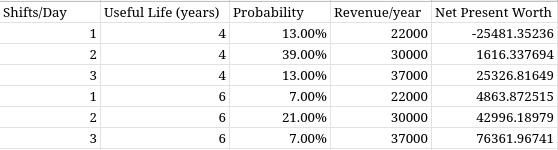
\includegraphics[width=0.8\textwidth]{q1}
    \caption{Net present worth by possibilities for question 1}
    \label{fig:q1}
\end{figure}

{\noindent\bf Question 1b.} The net present worth can be calculated as 
\[
NPW=P+A(P/A, 7\%, n)
\]
for each option. Doing so results in the last column of figure \ref{fig:q1}. 

{\noindent\bf Question 1c.} The optimistic scenario is that the useful life and revenue is maximized, which gives a present worth of \$76361.97 with probability 7\% (for 3 shifts/day and 6 years useful life). The pessimistic approach is that they are both minimized giving a net present worth of \$-25481.35 with probability 13\% (for 1 shift/day and 4 useful years). The most likely is the possibility with the highest probability, which from figure \ref{fig:q1} we can see is 2 shifts a day with a useful life of 4 years which gives a present net worth of \$1616.34 with probability 39\% (for 2 shifts/day and 4 years useful life). 

{\noindent\bf Question 2.} There are 6 different ways to role a 7 and 4 other ways to role an 8, for a total of 10. Since there are 36 possible outcomes this means that there's a $\frac{10}{36}$ chance of losing the bet and a $\frac{1}{36}$ chance of winning. The extra roles in between don't change the probabilities since they are independent and just trigger a restart. Thus the expected value is
\[
EV=10\cdot \frac{1}{10+1}-1=\$-0.09
.\]

{\noindent\bf Question 3.} First we consider D2. The expected value of A2 is clearly \$10000, whereas the expected value of A1 is $0.4\cdot 12000+0.6\cdot 8100=\$9660$. The expected value of option B is simply $0.4\cdot 9000+0.6\cdot 5000=\$6600$. The expected value of A is $0.6\cdot 4000+0.4\cdot 10000=\$6400$. Thus option B should be chosen because it has a higher expected value. 

{\noindent\bf Question 4.} Using excel 30 random samples were drawn from the distribution and plotted as seen in figure \ref{fig:q4}. The resulting net present worth was calculated using: 
\[
NPW=-P+45000 \cdot (P /A, 4\%, n)
.\]
Here P is the capital cost and n is the number of years. Note that the expected value and standard deviation shown in figure \ref{fig:q4} change every time the numbers are regenerated because the sample size isn't very big. 

\begin{figure}[htpb]
    \centering
    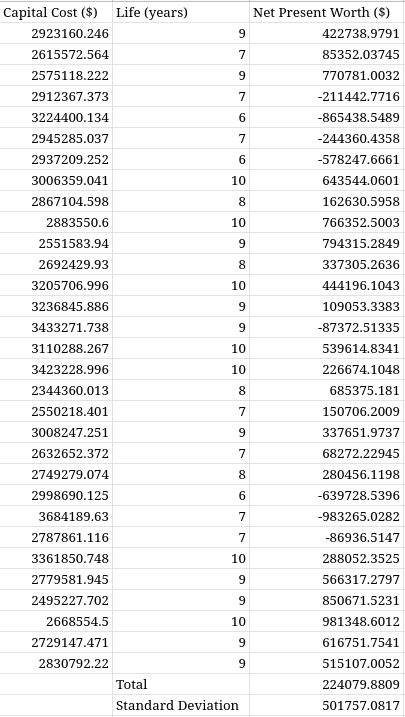
\includegraphics[width=0.8\textwidth]{q4}
    \caption{Random combinations of parameters for question 4. }
    \label{fig:q4}
\end{figure}

\end{document}
